%% 
%% 5. Vorlesung <2012-10-30 Tue>, Fortsetzung
%% 
%% Skript Differentialgeometrie im Wintersemester 12/13
%% Zur Vorlesung von Dr. Grensing am KIT Karlsruhe
%% 
%% Mitschrieb und Textsatz von Jan-Bernhard Kordaß.
%% 

\chapter{Tangentialbündel und Vektorfelder}

\begin{Dfn}[Tangentialbündel]
  Es sei $M$ eine glatte Mannigfaltigkeit. Die Menge $\T M = \dot \bigcup_{p \in M}\T_pM$ zusammen mit der sogenannten kanonischen Projektion $\pi \colon \T M \to M, \T_pM \ni X_p \mapsto p$ heißt das \CmMark[Tangential!-b\"undel]{Tangentialb"undel} von $M$.
\end{Dfn}

\section{Das Tangentialbündel als glatte Mannigfaltigkeit}

Es sei $(\phi, U)$ eine Karte von $M$. Setzt man $\T M|_U = \pi^{-1}(U) = \dot \bigcup_{p\in U}\T_pM$, so ist nach Satz \ref{satz-2-9}
die Abbildung
\begin{align*}
  & \overline \phi \colon \T M|_U \to \phi(U) \times \R^m \subset \R^{2m}\\
  &\T_p M \ni X_p = \sum \xi^i\pdifffrac[p]{}{x^i} \mapsto (\phi(p),\xi)
\end{align*}
bijektiv.
Es sei eine Topologie auf $\T M$ dadurch erklärt, dass eine Menge $V \subset \T M$ genau dann offen ist, wenn für alle Karten $(\phi, U)$ die Menge $\overline \phi(V \cap \T M|_U)$ offen in $\R^{2m}$ ist. Diese Topologie ist hausdorffsch und besitzt eine abzählbare Basis, da dies für $M$ und $\R^m$ gilt. Nach Konstruktion sind alle $\overline \phi$ Homöomorphismen. Ist $\mathcal A = \{(\phi, U\}$ ein $C^{\infty}$-Atlas von $M$, so definiert
\begin{align*}
  \overline A = \{(\overline \phi, \T M|_U) \mid (\phi, U) \in \mathcal A\}
\end{align*}
eine glatte Struktur auf $\T M$. Für Karten $(\phi, U), (\psi, V)$ von $M$ ist der Kartenwechsel
\[\begin{array}{ccc}
  \overline \psi \circ \overline \phi^{-1} \colon \phi(U \cap V) \times \R^m &\to& \psi(U \cap V) \times \R^m \\
  (x, \xi) &\mapsto& (\psi \circ \phi^{-1}(x),\D(\psi \circ \phi^{-1}|_x\xi),
\end{array}\]
$(X_p = \sum \xi^i \pdifffrac[p]{}{x^i})$ ist glatt. Damit trägt $\T M$ in kanonischer Weise eine glatte Struktur.
Darüber hinaus ist die kanonische Projektion $\pi \colon \T M \to M$ bezüglich dieser glatten Struktur eine Submersion. (Beweis: Übungsaufgabe)

Ist $N$ eine weitere glatte Mannigfaltigkeit und $\Phi \colon M \to N$ glatt, so ist $\Phi_{*} \colon \T M \to \T N, \ X_p \mapsto \Phi_{*p}X_p$ eine glatte Abbildung (ebensfalls Übungsaufgabe).

\begin{Dfn}
  Eine stetige Abbildung $X \colon M \to \T M$ mit $\pi \circ X = \Id_M$ heißt \CmMark{Vektorfeld} auf $M$.
  Ist $X$ glatt (als Abbildung zwischen glatten Mannigfaltigkeiten), so heißt $X$ ein \CmMark[Vektorfeld!glattes]{glattes Vektorfeld}.
\end{Dfn}

\begin{bem}
Ist $(\phi, U)$ eine Karte von $M$, so sind die Abbildungen $U \to \T M|_U, \ p \mapsto \pdifffrac[p]{}{x^{i}}$ glatte Vektorfelder (in der Karte $\overline \phi$ sind diese genau die Abbildungen $(x,e_i)$).

Ist $X$ ein glattes Vektorfeld, so gilt für jedes $u \in U$:
\begin{align*}
	X_U = \sum \xi^i(u) \pdifffrac[U]{}{x^i},
\end{align*}
wobei $\xi(u) = (\xi^1(u), \ldots, \xi^m(u))$ eine glatte Abbildung $U \to \R^m$ ist. Ein Vektorfeld ist genau dann glatte, wenn für jede Karte $(\phi, U)$ die Koeffizientenfunktionen $\xi^i(u)$ von $X_U = \sum \xi^i(u) \pdifffrac[U]{}{x^i}$ glatte Funktionen sind.
\end{bem}


%%% 
%%% 6. Vorlesung <2012-11-2 Fri>
%%% 

\begin{bsp}
  Betrachte die $n$-Sphäre $S^n \subset \R^{n+1}$ und deren Tangentialraum $\T_pS^n = p^{\perp}$.
  Ein glattes Vektorfeld auf $S^n$ ist also eine glatte Abbildung $X \colon S^n \to \R^{n+1}$ mit $X_p \perp p$.
  
  Es sei $n=2k-1$, dann ist
  \begin{align*}
    X \colon S^n \to \R^{n+1}, (x^1,y^1, \ldots, x^k,y^k) \mapsto (-y^1,x^1, \ldots, -y^k,x^k)
  \end{align*}
  ein glattes Vektorfeld auf $S^n$ ohne eine Nullstelle.
\end{bsp}

\begin{bem}
  Der \CmMark{Satz vom Igel} besagt gerade: Jedes glatte Vektorfeld auf einer Sphäre gerader Dimension hat eine Nullstelle.
\end{bem}

\begin{bem}
  Es bezeichne $\mathcal V(M)$ die Menge aller glatten Vektorfelder auf der Mannigfaltigkeit $M$. Der sogenannte \CmMark{Nullschnitt}:
  \begin{align*}
    \sigma \colon M \to \T M, p \mapsto 0_p \in \T_pM
  \end{align*}
  ist ein glattes Vektorfeld auf $M$.
  
  \emph{"Ubungsaufgabe:} Zeige dass der Nullschnitt eine Einbettung ist.
\end{bem}

\begin{bem}
  Sind $X,Y \in \mathcal V(M)$ und ist $g \in \C^{\infty}(M)$, so sind die punktweise Summe $X+Y$ und das Produkt $gX$ wieder ein glatte Vektorfelder auf $M$. Damit ist $\mathcal V(M)$ ein $\R$-Vektorraum beziehungsweise $C^{\infty}(M)$-Modul.
  
  Jedes Vektorfeld $X$ ist eine Derivation von $C^{\infty}(M)$:
  \begin{align*}
    X(fg)(p) = X(f)(p)g(p) + f(p) X(g)(p) = \left(gX(f) + fX(g)\right)(p).
  \end{align*}
  Es seien $X,Y \in \mathcal V(M)$ glatte Vektorfelder. Die \CmMark{Lieklammer} $[X,Y]$ von $X$ und $Y$ ist dann durch den folgenden Ausdruck definiert:
  \begin{align*}
    [X,Y](f)(p) = X_p(Yf)-Y_p(Xf).
  \end{align*}
\end{bem}

% Lemma 4.3
\begin{Lemma}
  Die Lieklammer ist eine schiefsymmetrische $\R$-bilineare Abbildung $\mathcal V(M) \times \mathcal V(M) \to \mathcal V(M)$. Es gilt die sogenannte \CmMark{Jacobiidentität}:
  \begin{align*}
    [X,[Y,Z]] + [Y,[Z,X]] + [Z,[X,Y]] = 0.
  \end{align*}
\end{Lemma}

\begin{bew}
  Es seien $X,Y \in \mathcal V(M)$, $f,g \in \C^{\infty}(M)$ und $p \in M$. Dann gilt:
  \begin{align*}
    [X,Y](fg)  = & X_p(Y(f)g + fY(g)) - Y_p(X(f)g+fX(g))\\
    = & X_p(Y(f))g(p) + \cancel{Y_p(f)X_p(g)} + \bcancel{X_p(f)Y(g)(p)} + f(p)X_p(Y(g))\\
    & - Y_p(X(f))g(p) - \bcancel{X_p(f)Y_p(g)} - \cancel{Y_p(f)X(g)(p)} - f(p)Y_p(X(g))\\
    = & (X_p(Y(f))-Y_p(X(f))g(p) + f(p)(X_p(Y(g))-Y_p(X(g))\\
    = & [X,Y]_p (f)g(p) + f(p)[X,Y]_p(g).
  \end{align*}
  \textcolor{red}{(nicht sicher ob ich die Durchstreichungen lassen oder rausnehmen soll)}
  Damit gilt $[X,Y] \in \mathcal V(M)$. Schiefsymmetrie und $\R$-Linearität gelten offensichtlich. Die Jacobiidentität sie als Übungsaufgabe überlassen (Nachrechnen!).
\end{bew}


% Lemma 4.4
\begin{Lemma}
  Es seien $X,Y \in \mathcal V(M)$ glatte Vektorfelder und $(\phi,U)$ eine Karte von $M$.
  Sind dann $X|_U = \sum \xi^i\pdifffrac{}{x^i}, \ Y|_U = \sum \eta^i \pdifffrac{}{x^i}$ und $[X,Y]|_U = \sum \zeta^i \pdifffrac{}{x^i}$ die ensprechenden lokalen Darstellungen, so gilt:
  \begin{align*}
    \zeta^j = \sum \left(\xi^i\pdifffrac{\eta^j}{x^i} - \eta^i \pdifffrac{\xi^j}{x^i} \right).
  \end{align*}
\end{Lemma} 

Der Beweis ist als Übungs überlassen.


\section{Flüsse}

\marginnote{\begin{tikzpicture}[scale=0.75]
    % \draw[step=0.25,gray!15] (-3,-1) grid (2,5); \draw[step=0.5,gray!30] (-3,-1) grid (2,5); \fill (0,0) circle(0.1); %Hilfsgitter
    \tikzschnuller{(0,3)}
    \draw[->] (0.25,2.25) -- (-0.5,2.25); \draw[->] (-1.5,2.25) -- (-2,1.75); \draw[->] (-2.5,1) -- (-1.75,1.5); \draw[->] (-1.5,0.75) -- (-0.25,1.5);
    \draw (-2,0.75) ..controls(-2,0.75) and ($(-1,0.75) - 0.5*(0.75,0.25)$).. (-1,0.75) ..controls($(-1,0.75) + (0.75,0.25)$) and (0,1.75).. (0,1.75);
    \draw[->] (-1,0.75) -- ($(-1,0.75) + (0.75,0.25)$); \draw[->] (-2,0.75) -- (-1.75,1);
  \end{tikzpicture}}
Was haben Vektorfelder mit Differentialgleichungen zu tun? Jedes glatte Vektorfeld $X$ definiert ein Anfangswertproblem
\begin{align*}
  \begin{cases}
    \dot \gamma(t) = X_{\gamma(t)}\\
    \gamma(0) = p
  \end{cases},
\end{align*}
oder in lokalen Koordinaten:
\begin{align*}
  \begin{cases}
    \dot \gamma(t) = \xi(\tilde \gamma(t))\\
    \tilde \gamma(0) = 0, \text{ falls } \phi(p) = 0,
  \end{cases}
\end{align*}
mit $\tilde \gamma = \phi \circ \gamma$ für eine Karte $(\phi,U)$ um $p$ und $X|_{\textcolor{red}{U}} = \sum \xi^i \pdifffrac{}{x^i}$.

% Definition 4.5
\begin{Dfn}
  Es sei $X \in \mathcal V(M)$ ein glattes Vektorfeld und $p \in M$, sowie $\calI \subset \R$ ein offenes, zusammenhängendes Intervall um $0$. Eine glatte Kurve $\gamma \colon \calI \to M$ mit
  \begin{align*}
    \dot \gamma(t) = X_{\gamma(t)}, \ \gamma(0) = p
  \end{align*}
  heißt \CmMark{Integralkurve} oder \CmMark{Trajektorie} von $X$ durch $p$.
\end{Dfn}

\begin{bem}
  Eine Kurve $\gamma$ ist genau dann Integralkurve von $X$ durch $p$, wenn für jede Karte $(\phi,U)$ die Kurve $\tilde \gamma = \phi \circ \gamma$ eine Lösung des (autonomen) Anfangswertproblems
  \begin{align*}
    \dot{\tilde \gamma} = \xi(\gamma(t)),  \ \tilde \gamma(0) = \phi(p)
  \end{align*}
  ist, wobei $X_U = \sum \xi^i \pdifffrac{}{x^i}$ gelte.

  Für jedes $p \in M$ ist somit (lokal) ein Anfangswertproblem gestellt. Gesucht ist eine \quot{simultane} Lösung all dieser Anfangswertprobleme, also eine Abbildung $(t,p) \mapsto \gamma(t,p) = \gamma^t(p)$ mit 
  \begin{align*}
    \begin{cases}
      \dot \gamma^t(p) = X_{\gamma^t(p)}\\
      \gamma^0(p) = p
    \end{cases}.
  \end{align*}
\end{bem}

% Satz 4.6
\begin{Satz}[Lokale Existenz und Eindeutigkeit]\label{satz-4-6}
  Es sei $U \subseteq \R^n$ offen und $\calI_{\epsilon}=(-\epsilon,\epsilon)$ und $F \colon \calI_{\epsilon} \times \R^n \to \R^n$ $C^k$-differenzierbar.
  Dann existiert für alle $x \in U$ eine Umgebung $V$ von $x$ in $U$ und ein $\delta > 0$, so dass
  \begin{enumerate}[label=(\roman*),leftmargin=*,widest=iii]
  \item Für alle $x \in V$ existiert eine $C^{k+1}$-Lösung $y_x\colon \calI_{\delta} \to V$, von $y_x'(t)=F(t,y(t))$ und $y_x(0) = x$.
  \item\label{satz-4-6-ii} Diese Lösung ist lokal eindeutig, das hei\ss t falls $\tilde y_x$ eine weitere Lösung auf $\calI_{\tilde\delta}$ ist, so gilt
    \begin{align*}
      y_x(t) = \tilde y_x(t) \text{ für alle } |t| \leq \min\{\delta, \tilde\delta\}.
    \end{align*}
  \item Die Abbildung 
    \begin{align*}
      y\colon \calI_{\delta} \times V \to U, \ (t,x) \mapsto y_x(t)
    \end{align*}
    ist $C^k$-differenzierbar.
  \end{enumerate}
\end{Satz}

Zum Beweis siehe Lang: "`Differential and Riemannian Manifolds"', 3. Auflage, 1995, Chapter IV.1, P.65\cite{lang1995differential}.

% Korollar 4.7
\begin{Kor}\label{korollar-4-7}\label{kor-4-7}
  Es sei $X \in \mathcal V(M)$ und $p \in M$. Dann existiert eine offene Umgebung $U$ von $p$, ein $\epsilon > 0$ und eine glatte Abbildung:
  \begin{align*}
    \gamma\colon(-\epsilon,\epsilon) \times U \to M
  \end{align*}
  so dass $t \mapsto \gamma^t(p)$ eine Integralkurve von $X$ durch $p$ ist. (Setze dann $F(t,x) = \xi(\phi^{-1}(x))$.)
\end{Kor}

% Korollar 4.8
\begin{Kor}\label{korollar-4-8}
  Sind $\gamma_1 \colon \calJ_1 \to M, \ \gamma_2 \colon \calJ_2 \to M$ Integralkurven eines Vektorfeldes $X \in \mathcal V(M)$ durch $p$, dann gilt $0 \in \calJ_1 \cap \calJ_2$ und $\gamma_1(0)= p = \gamma_2(0)$.
  Nach Satz \ref{satz-4-6} \ref{satz-4-6-ii} gilt dann $\gamma_1(t) = \gamma_2(t)$ für alle $t \in \calJ_1 \cap \calJ_2$. Damit ist
  \begin{align*}
    \gamma \colon \calJ_1 \cap \calJ_2, \ t \mapsto 
    \begin{cases}
      \gamma_1(t) & t \in \calJ_1\\
      \gamma_2(t) & t \in \calJ_2
    \end{cases}
  \end{align*}
  eine Integralkurve von $X$ durch $p$.
  Damit existiert für jedes $p \in M$ ein maximaler Definitionsbereich $\calI_p$ für Integralkurven von $X$ durch $p$; dieser ist offen.
\end{Kor}

\begin{dfn}
  Für $X \in \mathcal V(M)$ heißt die, wie im vorigen Korollar definierte, Familie maximaler Integralkurven
  \begin{align*}
    \gamma(t,p) = \gamma^t(p),\ t \in \calI_p
  \end{align*}
  der \CmMark{Fluss} des Vektorfeldes $X$.
  Seinen Definitionsbereich notiert man mit:
  \begin{align*}
    \mathcal D_X = \{(t,p) \in \R \times M \mid t \in \calI_p\}.
  \end{align*}
\end{dfn}

\begin{bem}
  Es gilt: $\gamma^0(\cdot) = \Id_M$. Ist $(s,p) \in \mathcal D_{X}$, so gilt
  \[ \difffrac[t=0]{}{t}(t \mapsto \gamma^{t+s}(p)) = X_{\gamma^s(p)}, \]
  also ist $t \mapsto \gamma^{t+s}(p)$ eine Integralkurve von $X$ durch $q = \gamma^s(p)$. Aus der Eindeutigkeit folgt damit:
  \begin{align*}
    \gamma^{t+s}(p) = \gamma^t(\gamma^s(p))
  \end{align*}
  f"ur alle $s, t$, $s+t \in \calI_p$, ferner gilt $\calI_q = \calI_p - s$. Kurz geschrieben: $\gamma^{t+s} = \gamma^t \circ \gamma^s$. Also definiert $\gamma$ einen \quot{lokalen Gruppenhomomorphismus} von $\R$ in $M^M$.
\end{bem}

% Satz 4.9
\begin{Satz}\label{satz-4-9}
  Ist $X \in \mathcal V(M)$ ein glattes Vektorfeld mit Fluss $\gamma$, so ist $\mathcal D_X$ eine offene Menge und sein Fluss $\gamma \colon \mathcal D_X \to M$ glatt.
\end{Satz}


%%% 
%%% 7. Vorlesung <2012-11-6 Tue>
%%% 

\begin{bem}[Erinnerung]
\textcolor{red}{TODO: Diesen Absatz aufräumen. (ich würde das komplett weglassen weil es bloß eine Wiederholung von der Woche davor ist -Aleks)}
Ist $X \in \mathcal V(M)$, $c$ Integralkurve von $X$ durch $p$, wenn $c(t) = X_{c(t)}$ maximales Existenzintervall $I_p$\\

%%% 
%%% TODO Abbildung 7-1
\textcolor{red}{Abbildung 7-1}
%%% 

\begin{align*}
	\gamma \colon \mathcal D_X = \{(t,p) \mid p \in M, t \in I_p\} \to M
\end{align*}
Fluß von $X$, wobei
\begin{align*}
	\dot \gamma^t = X_{\gamma^t(p)}, \gamma^0 = \Id_M.
\end{align*}
Für $f \in C^{\infty}$ gilt
\begin{align*}
	X_p(t) = \dot \gamma^t(pXf) = \difffrac[t=0]{}{t}(f \circ \gamma^t)(p).
\end{align*}
Aus der lokalen Eindeutigkeit folgt (für kleine Zeiten)
\begin{align*}
	\gamma^{s-t} = \gamma^s \circ \gamma^t.
\end{align*}
Für alle $t$ ist $\gamma^t$ (lokalaer) Diffeomorphismus mit Inversen $\gamma^{-t}$.
\end{bem}

\begin{bew}
Es sei $p \in M$ und $\calJ_p^{+}$ die Menge aller $t \geq 0$, für welche eine offene Umgebung $U$ von $[0,t] \times \{p\}$ in $\R \times M$ existiert, so dass $\gamma$ auf $U$ glatt ist.
\begin{itemize}
\item $\calJ_p^{+}$ ist ein Intervall,
\item $\calJ_p^{+} \subseteq \calJ_p \cap \R_{\geq 0}$
\item $0 \in \calJ_p^{+}$
\item $\calJ_p^{+}$ ist offen in $\R_{\geq 0}$.
\end{itemize}
Es bleibt zu zeigen, dass $\calJ_p^{+}$ abgeschlossen ist.

Es sei $s \in \overline \calJ_p^{+} \cap (\calJ_p \cap \R_{\geq 0}$ und $q = \gamma^s(p)$.\marginnote{\begin{tikzpicture}[scale=0.75,font=\tiny]
	%\draw[step=0.25,gray!15] (-3,-3) grid (3,3); \draw[step=0.5,gray!30] (-3,-3) grid (3,3); \fill (0,0) circle(0.1); %Hilfsgitter
	\draw[name path=kurve] (0,0) node[anchor=north west]{$\gamma^0(p) = p$} to[out=65,in=185] (2.75,2) node[anchor=north west]{$\gamma^s(p) = q$};
	\path[name path=senkrecht] (2.5,0) -- (2.5,3);
	\path[name intersections={of=kurve and senkrecht}];
	\fill (intersection-1) circle (0.05) node[anchor=south east] {$\gamma^t(p)$} (0,0) circle(0.05) (2.75,2) circle(0.05);
\end{tikzpicture}}
Dann existieren $\epsilon > 0$ und eine Umgebung $U$ von $q$, so dass $\gamma$ auf $(-\epsilon,\epsilon) \times U$ glatt ist.
Es sei $t \in \calJ_p^{+}$ mit $s-t < \epsilon$ und $\gamma^t(p) \in U$.
Nach Definition von $\calJ_p^{+}$ existiert eine offene Umgebung $V$ von $p$ in $M$ und $\delta > 0$, so dass $(-\delta,t+\delta)\times V \subseteq \mathcal D_X$ gilt und darauf $\gamma$ glatt ist.
Dann ist $V' = \left(\left.\gamma^t\right|_V\right)^{-1}(U) = \{p' \in V \mid \gamma^t(p') \in U\}$ eine offene Umgebung von $p$.
Für alle $p' \in V'$ gilt:
\begin{align*}
	r \mapsto
	\begin{cases}
		\gamma^r(p') & \text{ falls } r < t+\delta\\
		\gamma^{r-t}(\gamma^t(p')) & \text{ falls } r \in \textcolor{red}{(t-s,t+\epsilon)}
	\end{cases}.
\end{align*}
ist eine Integralkurve von $X$ durch $p'$.

Es gilt also $(-\delta,t+\epsilon) \subseteq \calJ_{p'}$ für alle $p' \in V'$ und somit $(-\delta,t+\epsilon) \times V' \subset \mathcal D_X$. An der obigen Darstellung sieht man, dass $\gamma$ darauf glatt ist.
Also gilt $s \in \calJ_p^{+}$. Analog argumentiert man für $\calJ_p^{-}$.
\end{bew}

% Definition 4.10
\begin{Dfn}[vollständiges Vektorfeld]
  Ein Vektorfeld auf $M$ heißt \CmMark{vollständig}, wenn der Definitionsbereich seines Flusses gleich $\R \times M$ ist.
\end{Dfn}

\begin{bem}
  Dies ist genau dann der Fall, wenn alle Integralkurven für alle Zeiten existieren. Ist $X \in \mathcal V(M)$ vollständig und bezeichnet $\gamma$ seinen Fluss, so ist jede $\gamma^t$ ein Diffeomorphismus von $M$ mit Inversen $\gamma^{-t}$.
\end{bem}

% Lemma 4.11
\begin{Lemma}
  Es sei $c \colon \calI \to M$ eine Integralkurve von $X \in \mathcal V(M)$ durch $p$ und $t_n \in \calI$ eine Folge, so dass die Grenzwerte $t_n \xrightarrow{n\to\infty} t_{\infty} \in \R$ und $c(t_n) \to q \in M$ existieren.
  
  Dann gilt $t_{\infty} \in \calI_{p}$ und $\gamma^{t_{\infty}}(p) = q$.
\end{Lemma}

\begin{bew}
  Nach Korollar \ref{korollar-4-7} existiert eine Umgebung $U$ von $q$ und $\epsilon > 0$, so dass auf $(-\epsilon,\epsilon) \times U$ ein lokaler Fluss von $X$ definiert ist.
  
  Wählt man $k$ so groß, dass $t_{\infty} - t_k < \epsilon$ gilt, so ist für $\overline q = c(t_k)$ und $t$ mit $|t-t_k| < \epsilon$ der Fluss $t \mapsto \gamma^{t-t_k}(\overline q)$ erklärt. Aus Korollar \ref{korollar-4-8} folgt, dass $\gamma^{t_k}(p) = c(t_k) = \overline q$ gilt.
  Damit ist die Kurve
  \begin{align*}
    \overline c(t) =
    \begin{cases}
      c(t) & \text{ für } t < t_{\infty}\\
      \gamma^{t-t_k}(\overline q) & \text{ falls } |t-t_k| < \epsilon
    \end{cases}
  \end{align*}
  eine glatte Fortsetzung von $c$ und eine Integralkurve von $X$ durch $p$.
  Insbesondere gilt $t_{\infty} < t_k + \epsilon$, also $t_{\infty} \in \calI_p$ und
  \begin{align*}
    \gamma^{t_{\infty}}(p)= \gamma^{t_{\infty}-t_k}(\gamma^{t_k}(p)) = \overline c(t_{\infty}) = \lim_{t\to t_{\infty}}c(t) = q.
  \end{align*}
\end{bew}

\begin{Bem}[Moral des obigen Lemmas]
  Integralkurven existieren für alle Zeiten oder aber sie verlassen jedes Kompaktum.
\end{Bem}

\begin{Kor}
Hat $X \in \mathcal V(M)$ kompakten Träger, so ist $X$ vollständig. Ist $M$ kompakt, os ist jedes glatte Vektorfeld vollständig.
\end{Kor}

\begin{bsp}
  Das Vektorfeld $X \colon \R \to \T\R, t \mapsto t^2\pdifffrac{}{t}$ ist nicht vollständig, denn $c(t) = (1-t)^{-1}$ ist die Integralkurve von $X$ durch $1$.
\end{bsp}


%\begin{bem}
Ist $\Phi \colon M \to N$ glatt, so ist $\Phi_{\ast} \colon \T M \to \T N$ glatt.\marginnote{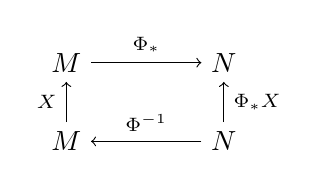
\begin{tikzpicture}[scale=1]
	%\draw[step=0.25,gray!15] (-3,-1) grid (3,1); \draw[step=0.5,gray!30] (-3,-1) grid (3,1); \fill (0,0) circle(0.1); %Hilfsgitter
	\def\hor{1}
	\def\vert{0.5}
	\node (0) at (-\hor,\vert) {$\T M$}; \node (1) at (\hor,\vert) {$\T N$}; \node (2) at (\hor,-\vert) {$N$}; \node (3) at (-\hor,-\vert) {$M$};
	\draw[->] (0) --node[above,font=\scriptsize]{$\Phi_*$} (1); \draw[->] (2) --node[right,font=\scriptsize]{$\Phi_*X$} (1); \draw[->] (2) --node[above,font=\scriptsize]{$\Phi^{-1}$} (3); \draw[->] (3) --node[left,font=\scriptsize]{$X$} (0);
\end{tikzpicture}}
Ist $\Phi$ ein Diffeomorphismus, so ist $\Phi^{-1}$ glatt und $q \mapsto (\Phi_{\ast}X)_q = \Phi_{*\Phi^{-1}(q)}X_{\Phi^{-1}(q)}$ ist ein glattes Vektorfeld auf $N$. Es gilt für $f \in C^{\infty}(N)$:
\begin{align*}
  (\Phi_{\ast}X)(f)(q) = X_{\Phi^{-1}(q)}(f \circ \Phi).
\end{align*}
%\end{bem}


% Lemma 4.13
\begin{Lemma}
  Es sei $X \in \mathcal V(M)$, $\Phi \colon M \to N$ ein Diffeomorphismus und es bezeichne $\gamma$ den Fluss von $X$ und $\mathcal D_X$ seinen (maximalen) Definitionsbereich.
Dann ist
\begin{align*}
  \{(t,q) \mid (t,\Phi^{-1}(q)) \in \mathcal D_X\} \to N \colon (t,q) \mapsto \Phi \circ \gamma^t \circ \Phi^{-1}(q)
\end{align*} 
der Fluss von $\Phi_{*}X$.
\end{Lemma}

\begin{bew}
Für $f \in \C^{\infty}(N)$ und $q \in N$ gilt
\begin{align*}
	(\Phi_{\ast}X)(f)(q) & = X_{\Phi^{-1}(q)}(f \circ \Phi)\\
	& = \difffrac[t=0]{}{t} (f \circ \Phi)(\gamma^t(\Phi^{-1}(q)))\\
	& = \difffrac[t=0]{}{t}f(\underbrace{\Phi \circ \gamma^t \circ \Phi^{-1}}_{\text{Fluss von }\Phi_{*}X}(q)).
\end{align*}
\end{bew}

%\begin{Bem}
\emph{Erinnerung:} $\frac{1}t(F(x+tv)-F(x))$ oder für $c$ mit $c(0) = x, \dot c(0) = v$: $\frac{1}t(F(c(t))-F(x))$.

Nun seien $X,Y \in \mathcal V(M)$.
\begin{center}\begin{tikzpicture}[font=\scriptsize]
	%\draw[step=0.25,gray!15] (-6,-1) grid (6,5); \draw[step=0.5,gray!30] (-6,-1) grid (6,5); \fill (0,0) circle(0.1); %Hilfsgitter
	\draw[name path=kurve] (-3,0) ..controls(-3,0) and (-2.75,1).. (0,1.5) node[below] {$\gamma^{t}(p)$} ..controls(1.5,1.75) and (2.5,2.5).. (2.5,2.5) node[anchor=north west] {$\gamma^{(\cdot)}(p)$};
	
	\fill (0,1.5) circle(0.05); \draw[->] (0,1.5) --node[left]{$y_{\gamma^t(p)}$} (1,2.5);
	
	\path[name path=senkrecht] (-2,0) -- (-2,3);
	\path[name intersections={of=kurve and senkrecht}];
	\fill (intersection-1) circle(0.05); \draw[->] (intersection-1) node[below] {$p$} --node[left]{$y_p$} (-2.5,2.5);
	
	\node[font=\normalsize] at (0,0) {$\gamma^t$};
\end{tikzpicture}\end{center}
Im Allgemeinen liegen $y_{\gamma^t(p)}$ und $y_p$ in unterschiedlichen Tangentialräumen.
Da aber $\gamma^t$ (für kleine Zeiten) ein (lokaler) Diffeomorphismus ist, gilt
\begin{align*}
  \gamma_{*}^{-t}(y_{\gamma^t(p)})-(\gamma_{*}^{-t}y)_p \in \T_pM.
\end{align*}
Die Differenz $(\gamma_{*}^{-t}y)_p - y_p$ ist also wohldefiniert. \textcolor{red}{(Ich bin mir nicht sicher ob die $y$ gro\ss  oder klein geschrieben sein sollen -Aleks)}
%\end{Bem}

\begin{Dfn}
  Es seien $X,Y \in \mathcal V(M)$ und $\gamma$ der Fluss von $X$.
Das durch 
\begin{align*}
  p \mapsto \lim_{t\to 0}\frac{1}t\left(\left(\gamma_{*}^{-t}y\right)_p-y_p\right)
\end{align*}
definierte glatte Vektorfeld heißt \CmMark{Lieableitung} von $Y$ längs $X$. Man schreibt $\mathcal L_XY$.
\end{Dfn}

%\begin{Bem}
Die Kurve $(\gamma_{*}^{-t}y)_p$ in $\T_pM$ ist glatt und $(\mathcal L_XY)_p = \difffrac[t=0]{}{t}(\gamma_{*}^{-t}Y)_p$. Dass $\mathcal L_XY$ glatt ist, rechnet man entweder in lokalen Koordinaten nach oder benutzt den folgenden Satz.
%\end{Bem}

% Satz 4.15
\begin{Satz}
  Für $X,Y \in \mathcal V(M)$ gilt:
  \begin{align*}
    \mathcal L_XY = [X,Y].
  \end{align*}
\end{Satz}

\begin{bew}
Es seinen $X,Y \in \mathcal V(M)$, $f \in \C^{\infty}(M)$ und $\gamma$ der Fluss von $X$.

Es ist zu zeigen: $[X,Y]_p(f) = \lim_{t \to \infty} \frac{1}{t}\left((\gamma_{*}^{-t}y)_p(f)-y_p(f)\right)$.
Dazu sei (um $(0,p)$)
\begin{align*}
  h(t,q) = f(\gamma^{-t}(q))-f(q) \text{ und } g_t(q) = \int_0^1 h'(ts,q)ds.
\end{align*}
Dann gilt:
\begin{align*}
  tg_t(q) = \int_0^1h'(ts,q)(t)ds = \int_0^th' = h(t,q) - h(0,q) = f(\gamma^{-t}(q)) - f(q)
\end{align*}
also $f \circ \gamma^t = f + tg_t$ und 
\begin{align*}
  g_0(q) = \lim_{t \to 0} \frac{tg_t(q)}{t} = \lim_{t \to 0}\frac{1}t\left(f(\gamma^{-t}(q))-f(q)\right) = \difffrac[t=0]{}{t}\left(f \circ \gamma^{-t}\right)(q) = -X_q(f)
\end{align*}
Betrachte:
\begin{align*}
  \left(\gamma_{*}^{-t}y\right)_p(f) = y\left(f \circ \gamma^{-t}\right)\left(\gamma^t(p)\right) = y(f)\left(\gamma^t(p)\right) + ty_{g_t}\left(\gamma^t(p)\right).
\end{align*}
Es folgt:
\begin{align*}
  \left(L_XY\right)_q(f) & = \lim \frac{1}t \left((\gamma_{*}^{-t}y)_p(f) - y_p(f)\right)\\
& = \lim_{t\to 0} \frac{1}t \left(yf(\gamma^t(p))-y_p(f)\right) + \lim_{t\to 0} y_{g_t}\left(\gamma^t(p)\right)\\
& = \difffrac[t=0]{}{t}\left(yf \circ \gamma^t\right)(p) + yg_0(p)\\
& = X_p(yf) - y_p(Xf) = [X,Y]_p(f).
\end{align*} 
\end{bew}


%%%
%%% 8. Vorlesung <2012-11-9 Fri>
%%% 

% Satz 4.16
\begin{Satz}
  Die Lieklammer $[X,Y]$ zweier Vektorfelder $X,Y \in \mathcal V(M)$ verschwindet genau dann, wenn ihre Flüsse (lokal) kommutieren, i.e.
  \begin{align*}
    \gamma_X^s \circ \gamma_Y^t = \gamma_Y^t \circ \gamma_X^s.
  \end{align*}
\end{Satz}

Der Beweis sei als Übungsaufgabe überlassen.

Es seien $X,Y \in \mathcal V(M)$ und $\Phi \colon M \to N$.
Bezeichnet $\gamma$ den Fluss von $X$, so gilt
\begin{align*}
  [\Phi_{\ast}X,\Phi_{\ast}Y] & = \mathcal L_{\Phi_{\ast}X} \Phi_{\ast}Y\\
  & = \difffrac[t=0]{}{t}\left(\Phi_{\ast} \circ \gamma_{\ast}^{-t} \circ \Phi_{\ast}^{-1}(\Phi_{\ast}Y)\right)\\
  & = \difffrac[t=0]{}{t} \left(\Phi_{\ast} \circ \gamma_{\ast}^{-t}Y\right) 
  = \Phi_{\ast}\left(\difffrac[t=0]{}{t}\gamma_{\ast}^{-t}Y\right)\\
  & = \Phi_{\ast}(\mathcal L_XY) = \Phi_{\ast}[X,Y].
\end{align*}
Man erhält einen alternativen Beweis der Jacobiidentität.


\begin{bew}
  Es seien $X,Y, Z \in \mathcal V(M)$ und $\gamma$ der Fluss von $X$.
  Dann gilt:
  \begin{align*}
    [X,[Y,Z]] & = \mathcal L_X[Y,Z] 
    = \difffrac[t=0]{}{t}\left(\gamma_{\ast}^{-t}[Y,Z]\right)\\
    & = \difffrac[t=0]{}{t}\left[\gamma_{\ast}^{-t}Y,\gamma_{\ast}^{-t}Z\right]\\
    & = \left[\difffrac[t=0]{}{t} \gamma_{\ast}^{-t}Y,Z\right] + \left[Y, \difffrac[t=0]{}{t}\gamma_{\ast}^{-t}Z\right]\\
    & = [\mathcal L_XY,Z] + [Y,\mathcal L_XZ]\\
    & = [[X,Y],Z] + [Y,[X,Z]]\\
    & = -[Z,[X,Y]] - [Y,[Z,X]].
  \end{align*}
\end{bew}

%%% Local Variables: 
%%% mode: latex
%%% TeX-master: "../skript-diffgeom"
%%% End: 
